\chapter*{
    \begin{center}
        \vspace{-2.6cm}
        {\fontsize{20}{26}\selectfont Annexe E : Interfaces de l'application AutoTest}
    \end{center}
}
\addcontentsline{toc}{chapter}{Annexe E : Interfaces de l'application AutoTest}
\vspace{-2.3cm}
\begin{justify}
    Cette annexe présente les interfaces de la nouvelle application AutoTest, organisées par release. Elles ont été repensées et améliorées à partir des observations faites sur la version initiale (voir Annexe A), dans une démarche d’optimisation de l’ergonomie et de l’expérience utilisateur.
    
    \textbf{\fontsize{16}{19}\selectfont   Release 1} :\\
            Cette première version pose les bases fondamentales du projet et prépare le terrain pour les développements futurs.  
            \begin{enumerate}[label=\Alph*.]
                \item \textbf{Sprint 1.1: Initialisation, authentification et gestion des permissions}  \\
                Ce sprint marque le démarrage du projet. Il comprend la structuration de l'application, la mise en place d’un système d’authentification sécurisé basé sur JWT, la gestion des rôles et des permissions, ainsi que le développement des premières interfaces publiques telles que la page d’accueil et le formulaire de contact. Les interfaces suivantes ont été conçues :
                \begin{figure}[H]
                    \centering
                    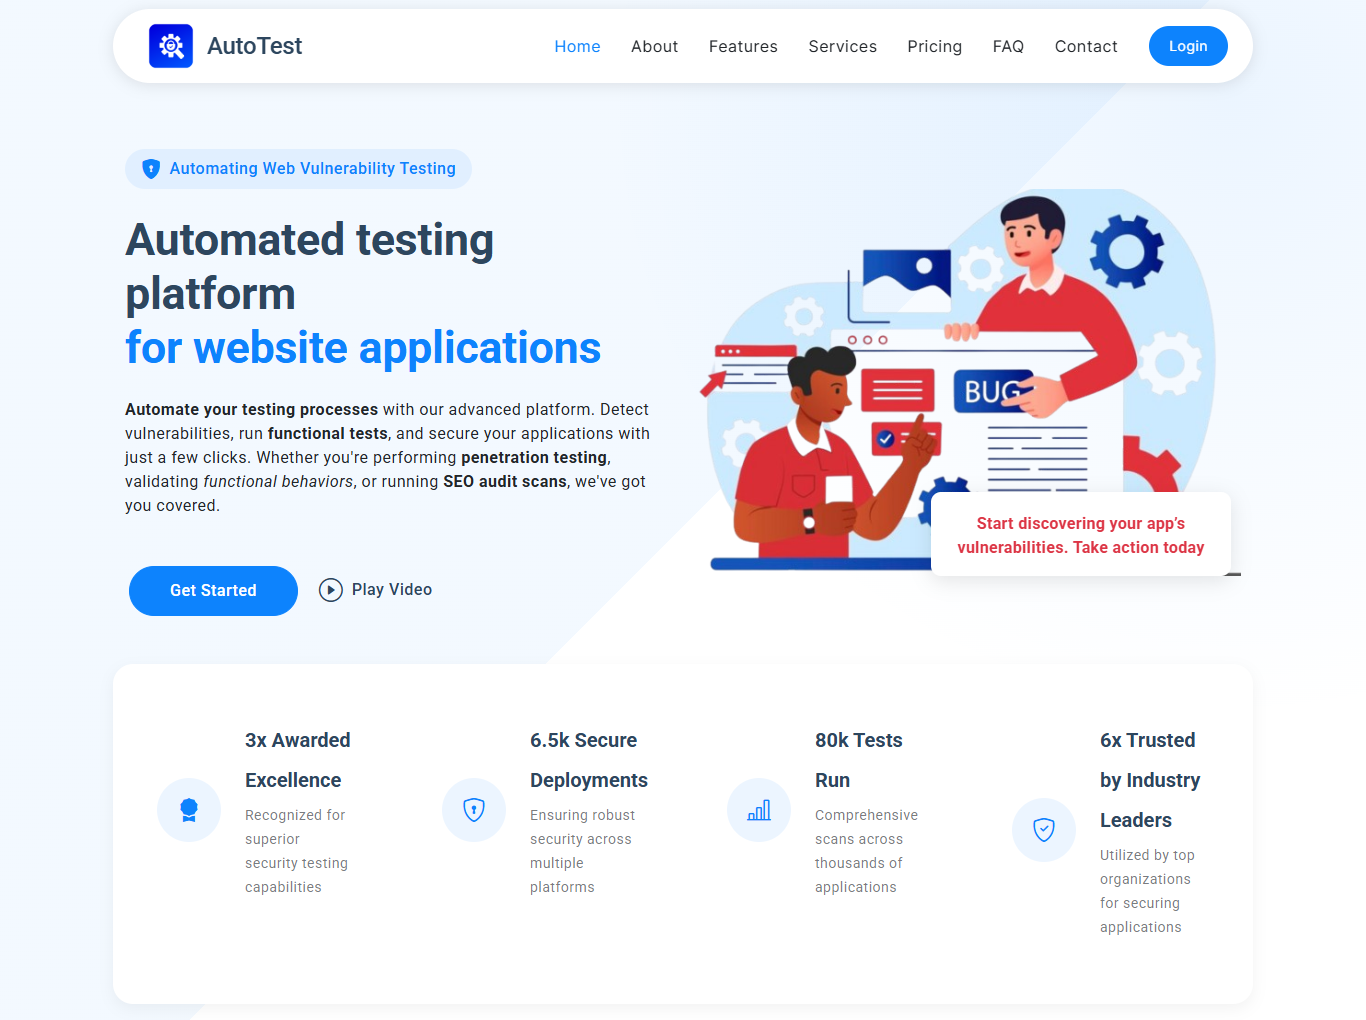
\includegraphics[width=\linewidth]{chapitres/ch3Sp1/section/sprint1/img/interface/acceuil-page.png}
                    \caption{Interface de la page d’accueil}
                    \label{fig:accueil}
                \end{figure}
                \begin{figure}[H]
                    \centering
                    \begin{minipage}[b]{0.495\linewidth}
                        \centering
                        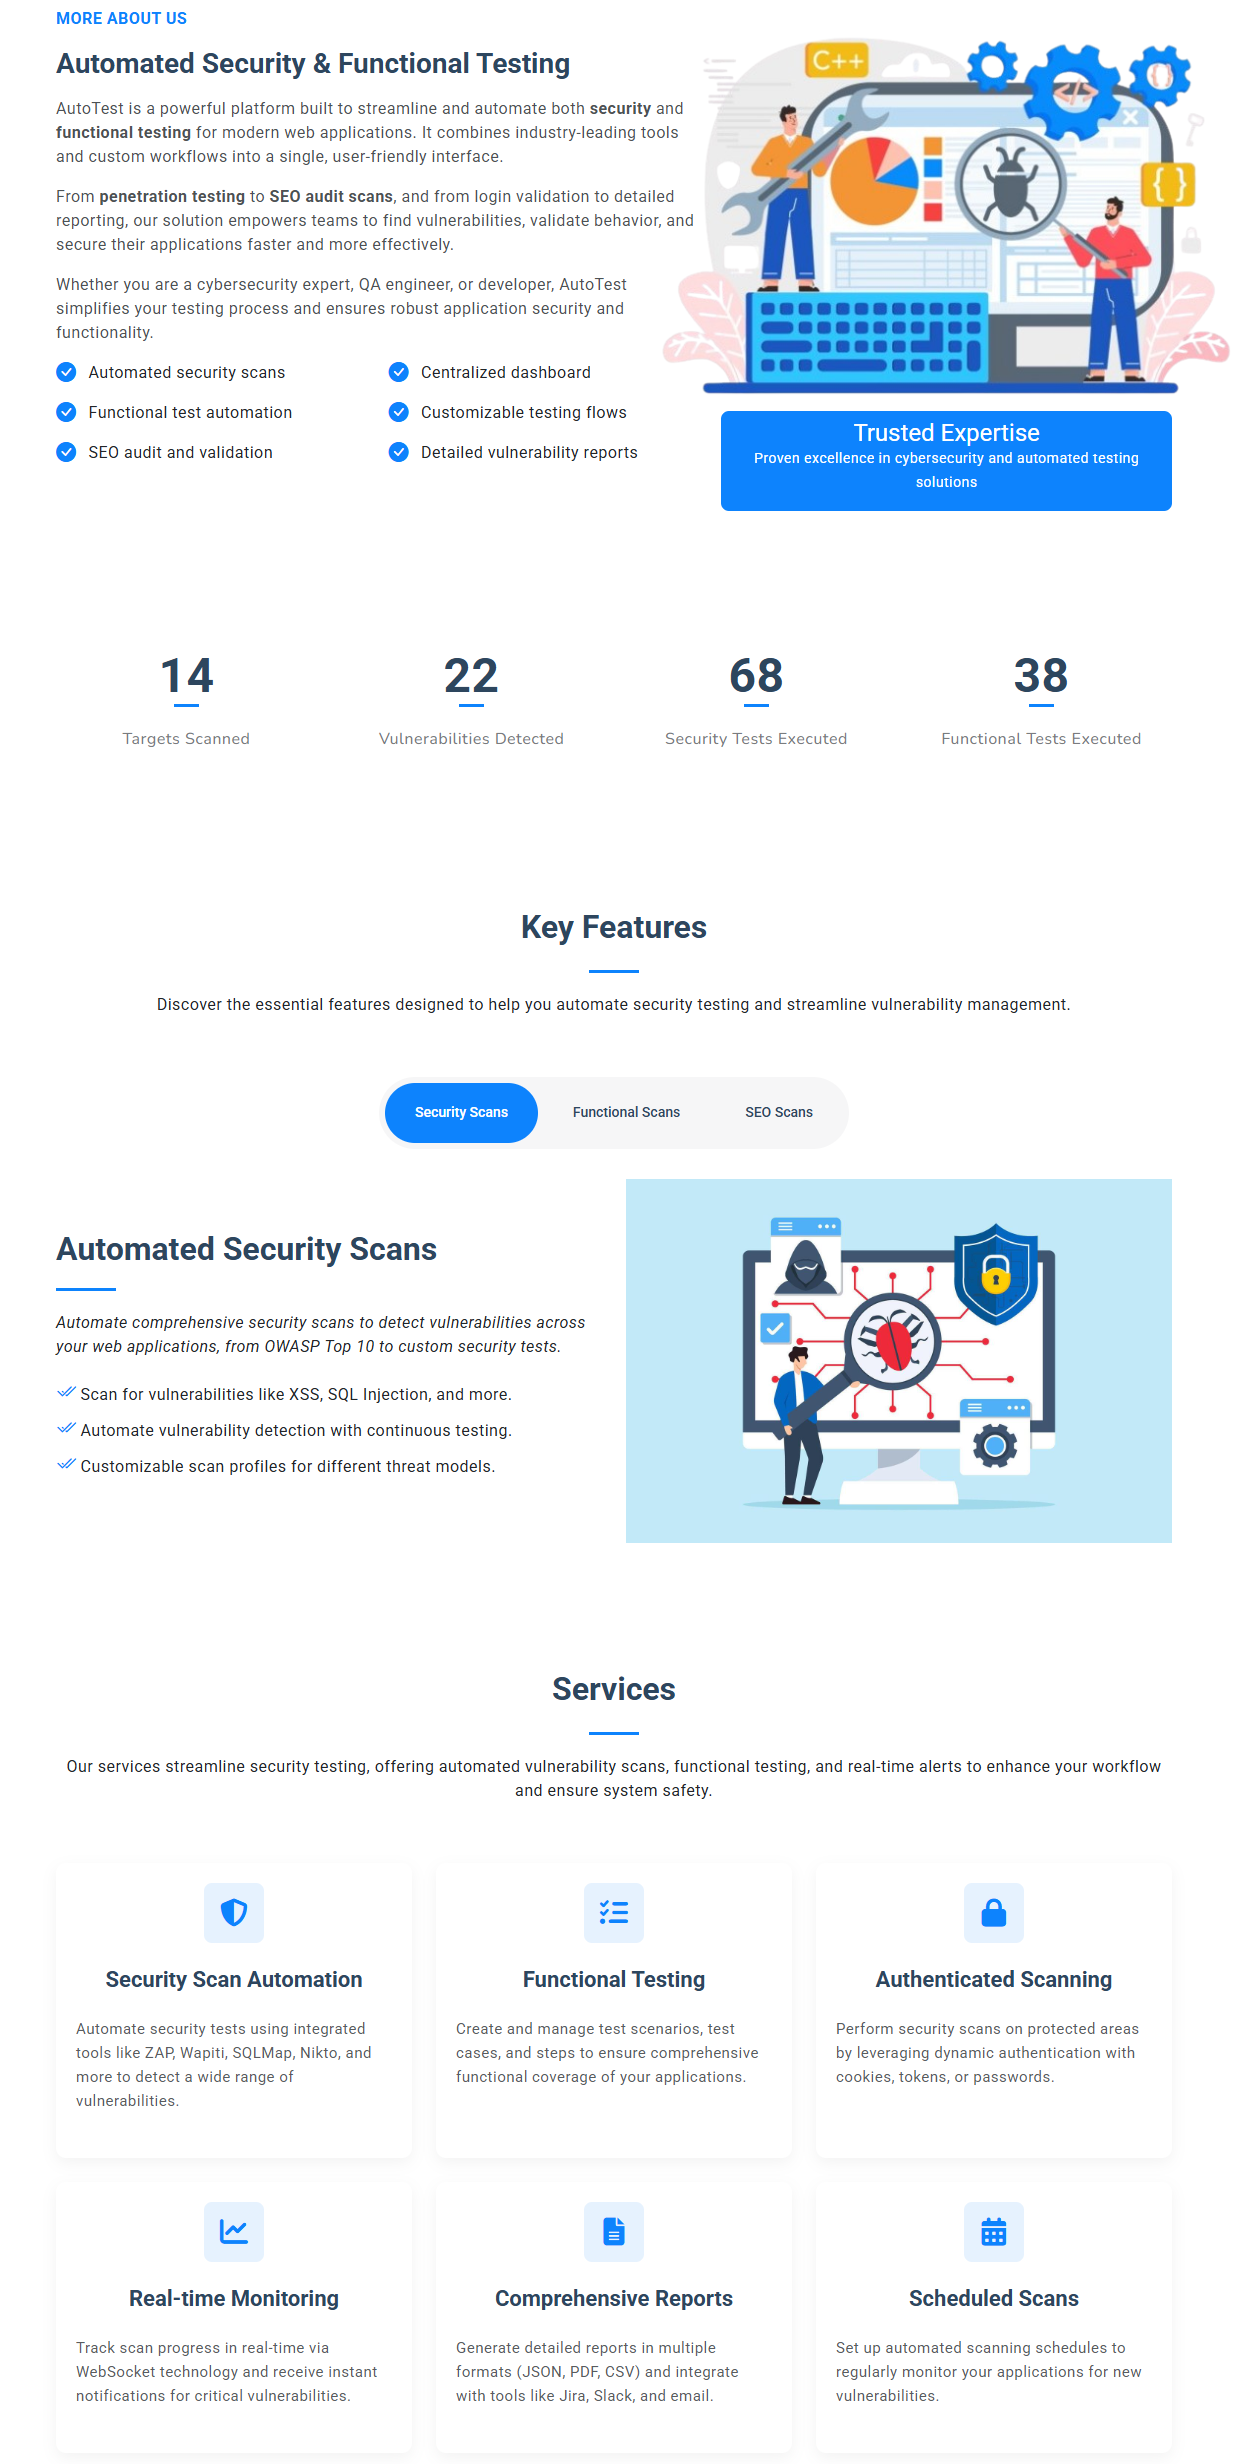
\includegraphics[width=\linewidth]{chapitres/ch3Sp1/section/sprint1/img/interface/a1.png}
                    \end{minipage}
                    \hfill
                    \begin{minipage}[b]{0.495\linewidth}
                        \centering
                        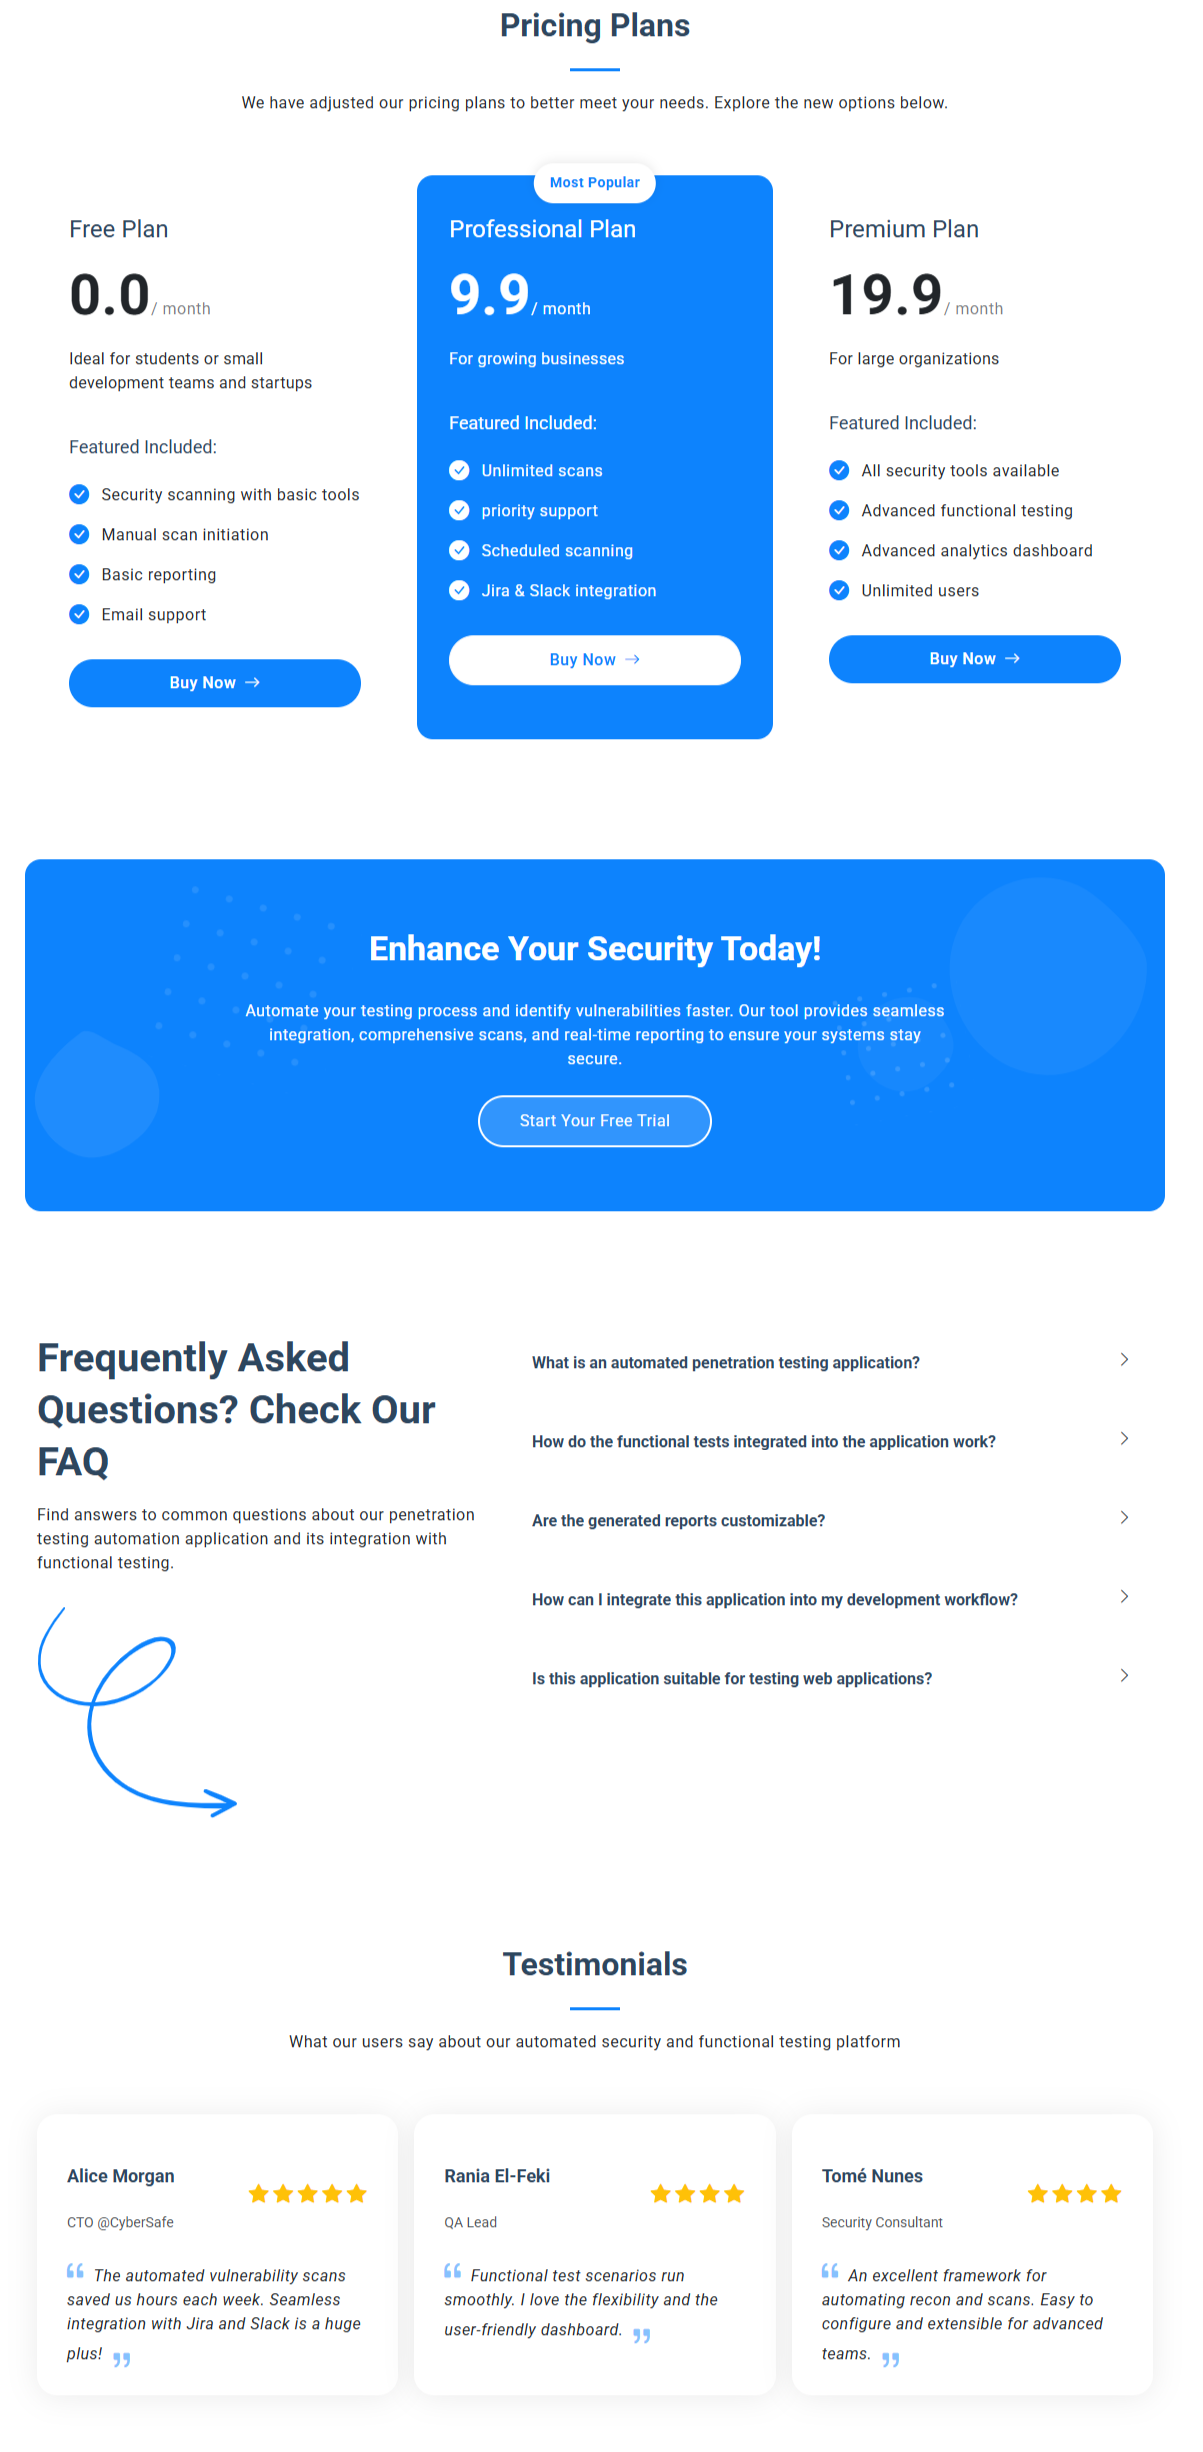
\includegraphics[width=\linewidth]{chapitres/ch3Sp1/section/sprint1/img/interface/a2.png}
                    \end{minipage}
                    \caption{\centering Autres sections de la page d’accueil}
                    \label{fig:accueil2}
                \end{figure}
                \vspace{-0.3cm}
                \begin{figure}[H]
                    \centering
                    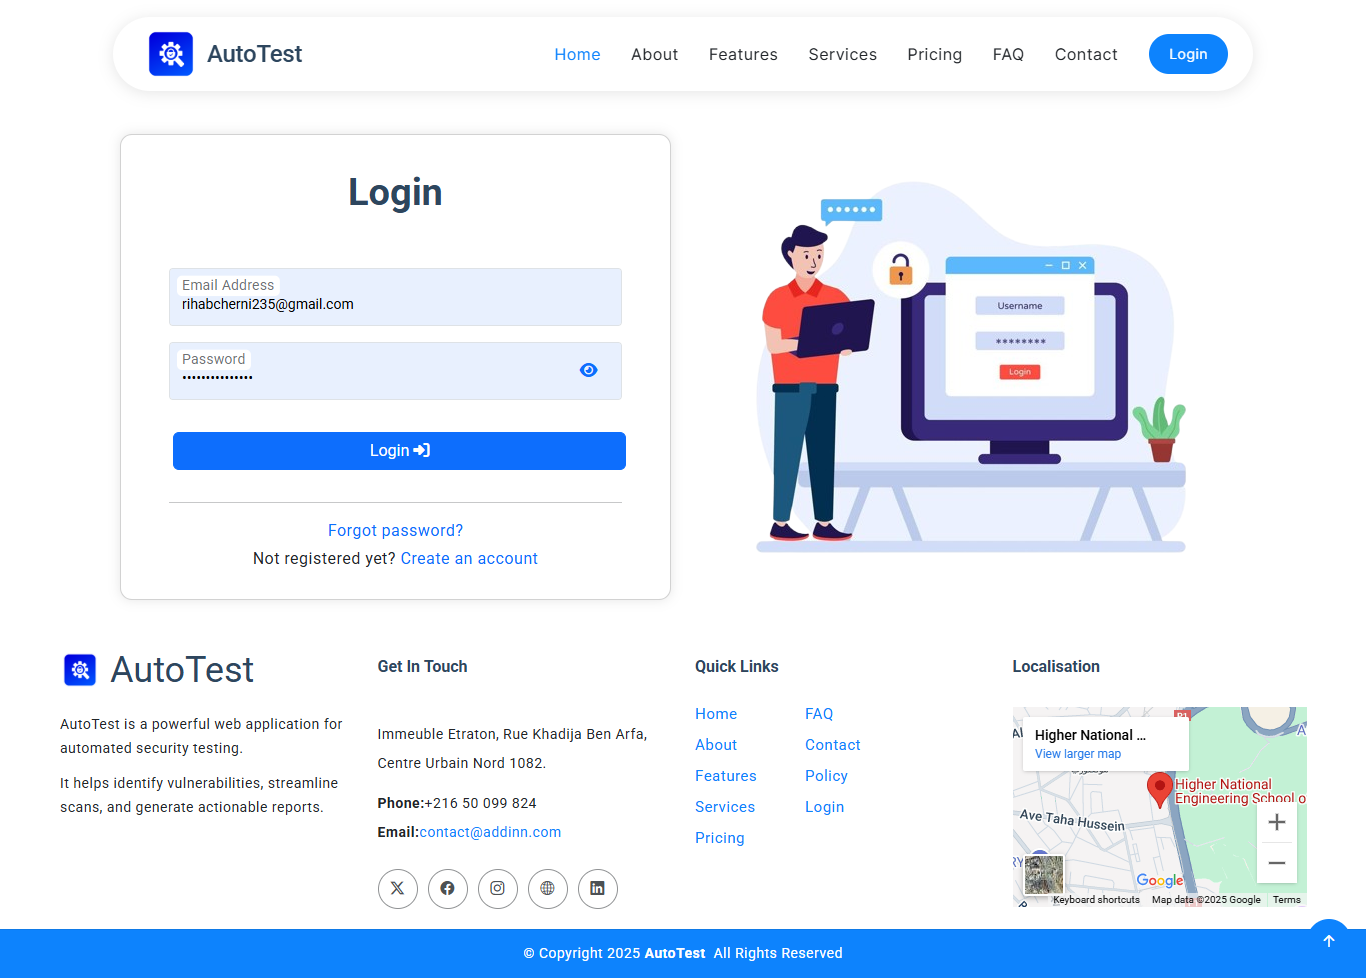
\includegraphics[width=0.95\linewidth]{chapitres/ch3Sp1/section/sprint1/img/interface/login.png}
                    \caption{Interface de connexion}
                    \label{fig:login}
                \end{figure}
                \vspace{-0.3cm}
                \begin{figure}[H]
                    \centering
                    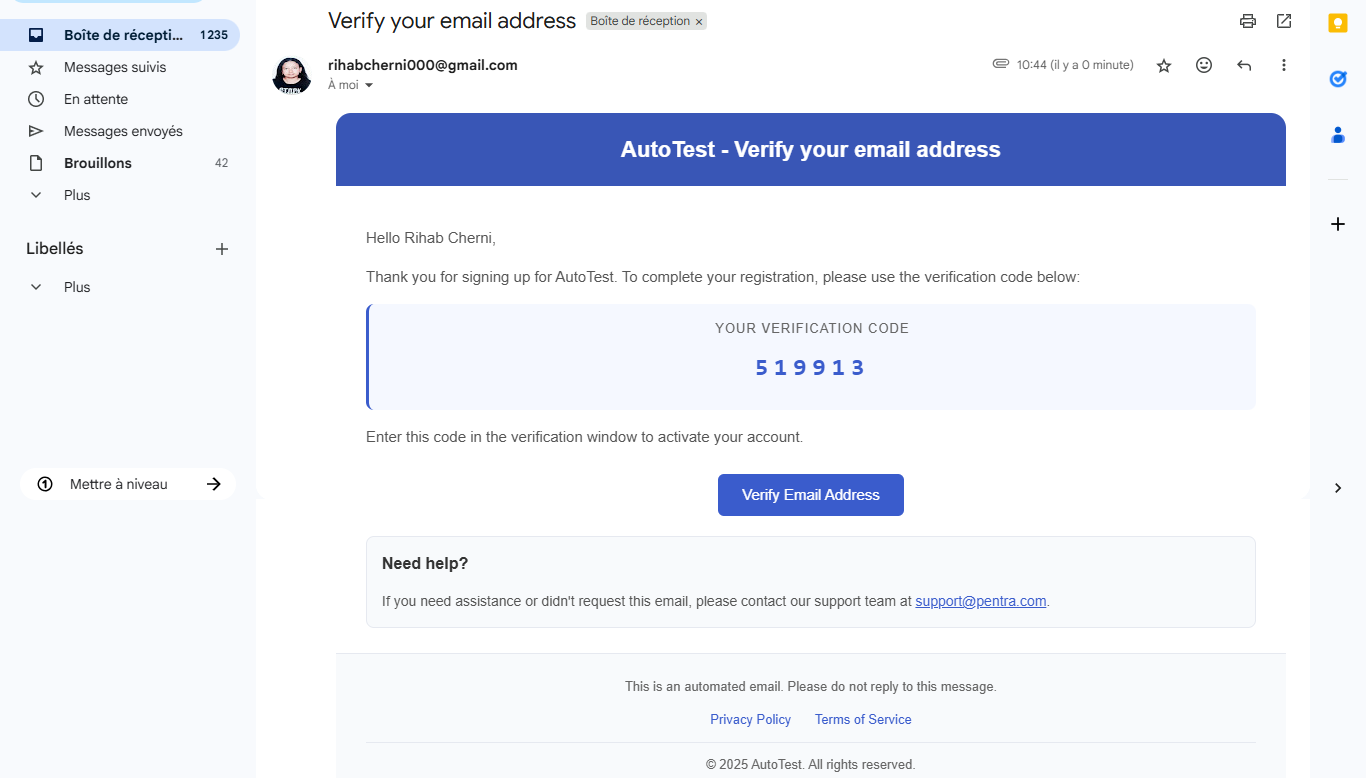
\includegraphics[width=\linewidth]{chapitres/ch3Sp1/section/sprint1/img/interface/email-verif.PNG}
                    \caption{\centering E-mail contenant le code OTP de vérification du compte}
                    \label{fig:email-verif}
                \end{figure}
                \vspace{-0.6cm}
                \begin{figure}[H]
                    \centering
                    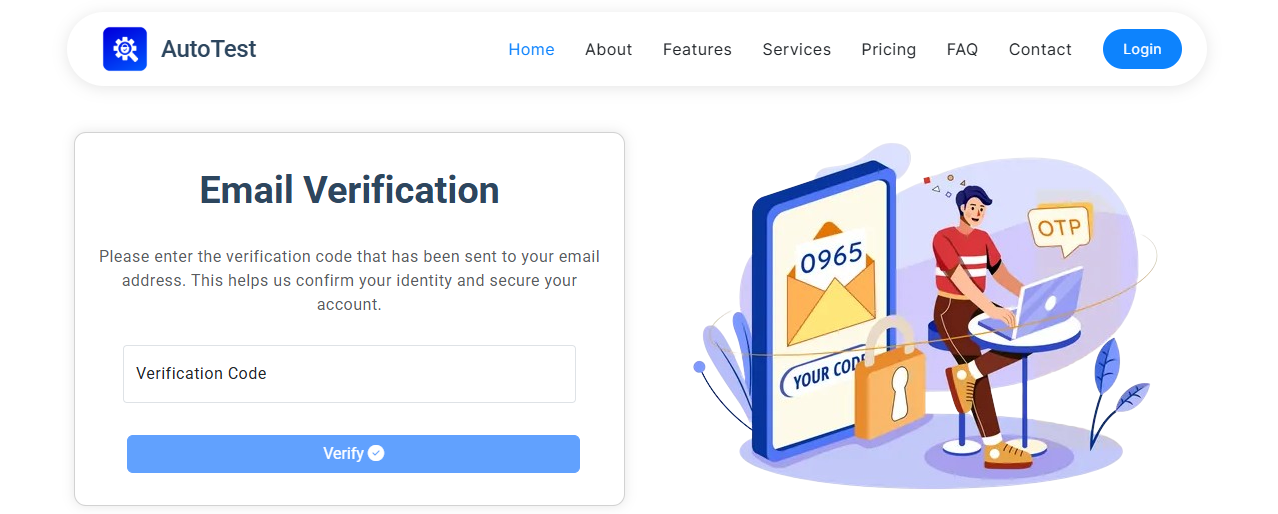
\includegraphics[width=\linewidth]{chapitres/ch3Sp1/section/sprint1/img/interface/email-verification.png}
                    \caption{\centering Interface de saisie du code OTP pour la vérification du compte}
                    \label{fig:email-verification}
                \end{figure}
                \vspace{-0.6cm}
                \begin{figure}[H]
                    \centering
                    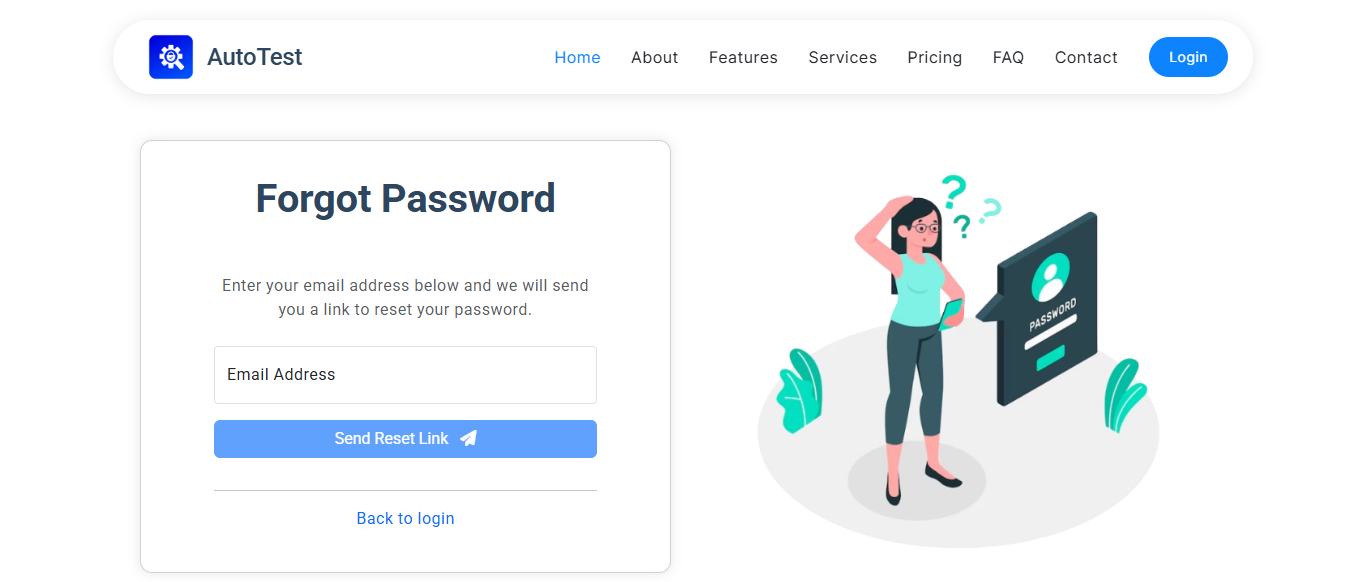
\includegraphics[width=\linewidth]{chapitres/ch3Sp1/section/sprint1/img/interface/forgot-password.png}
                    \caption{\centering Interface de récupération du mot de passe oublié}
                    \label{fig:forgot-password}
                \end{figure}
                \vspace{-0.6cm}
                \begin{figure}[H]
                    \centering
                    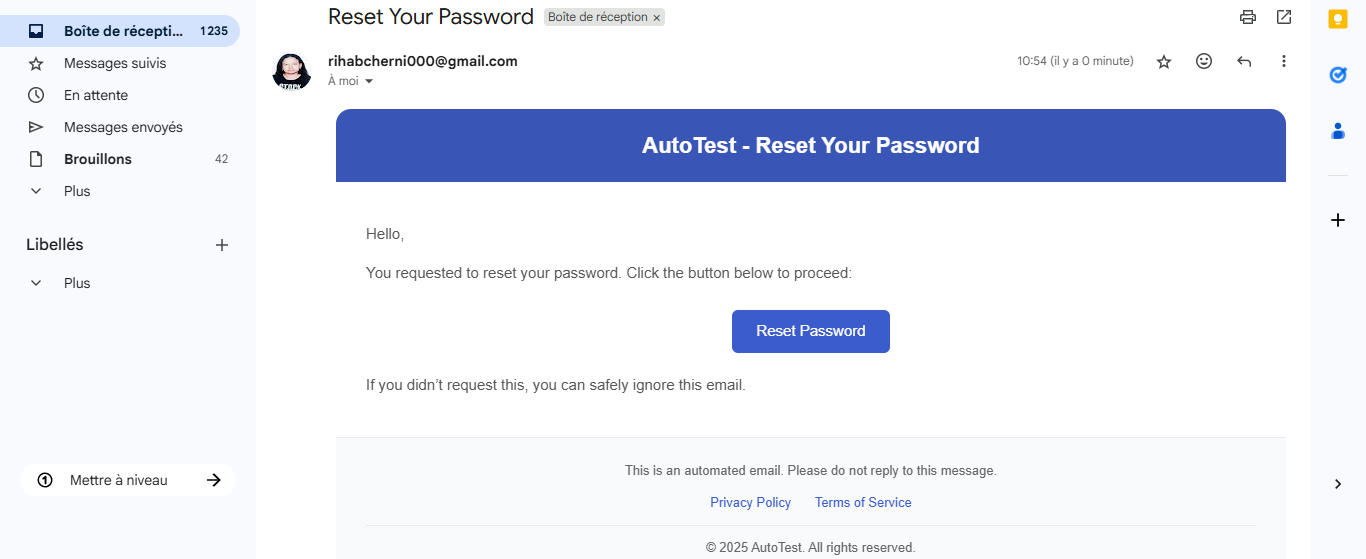
\includegraphics[width=\linewidth]{chapitres/ch3Sp1/section/sprint1/img/interface/reset-password-email.png}
                    \caption{\centering Confirmation d’envoi de l’e-mail de réinitialisation}
                    \label{fig:reset-password-email}
                \end{figure}
                \vspace{-0.6cm}
                \begin{figure}[H]
                    \centering
                    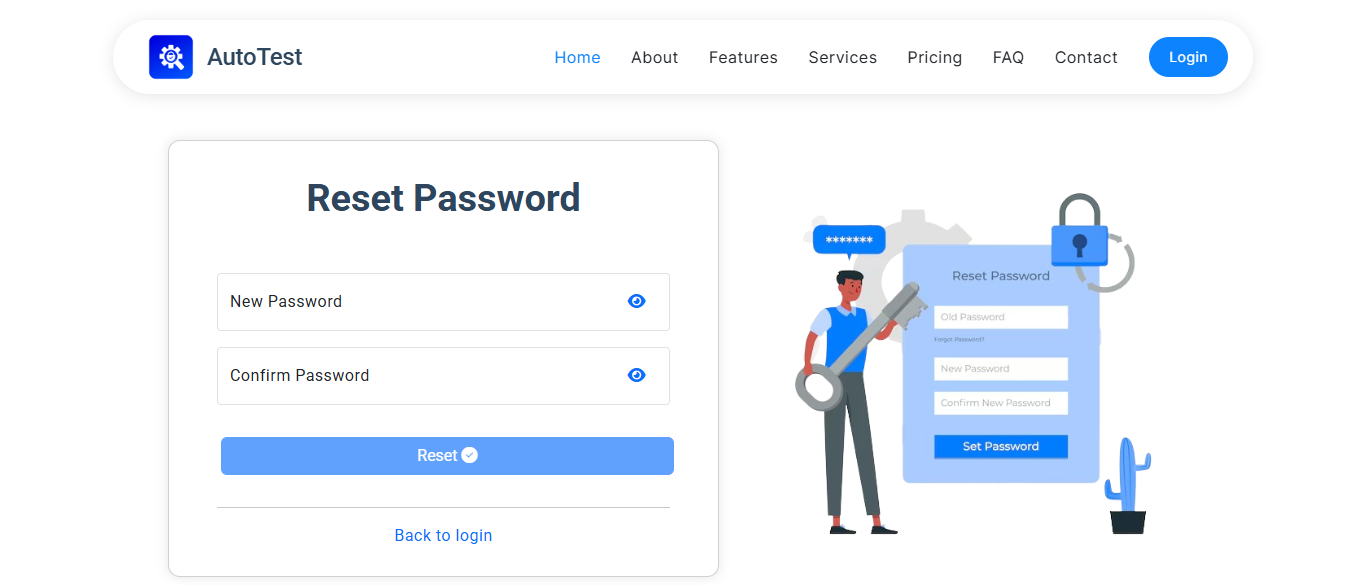
\includegraphics[width=\linewidth]{chapitres/ch3Sp1/section/sprint1/img/interface/reset-password.PNG}
                    \caption{\centering Interface de réinitialisation du mot de passe}
                    \label{fig:reset-password}
                \end{figure}
                \vspace{-0.6cm}
                \begin{figure}[H]
                    \centering     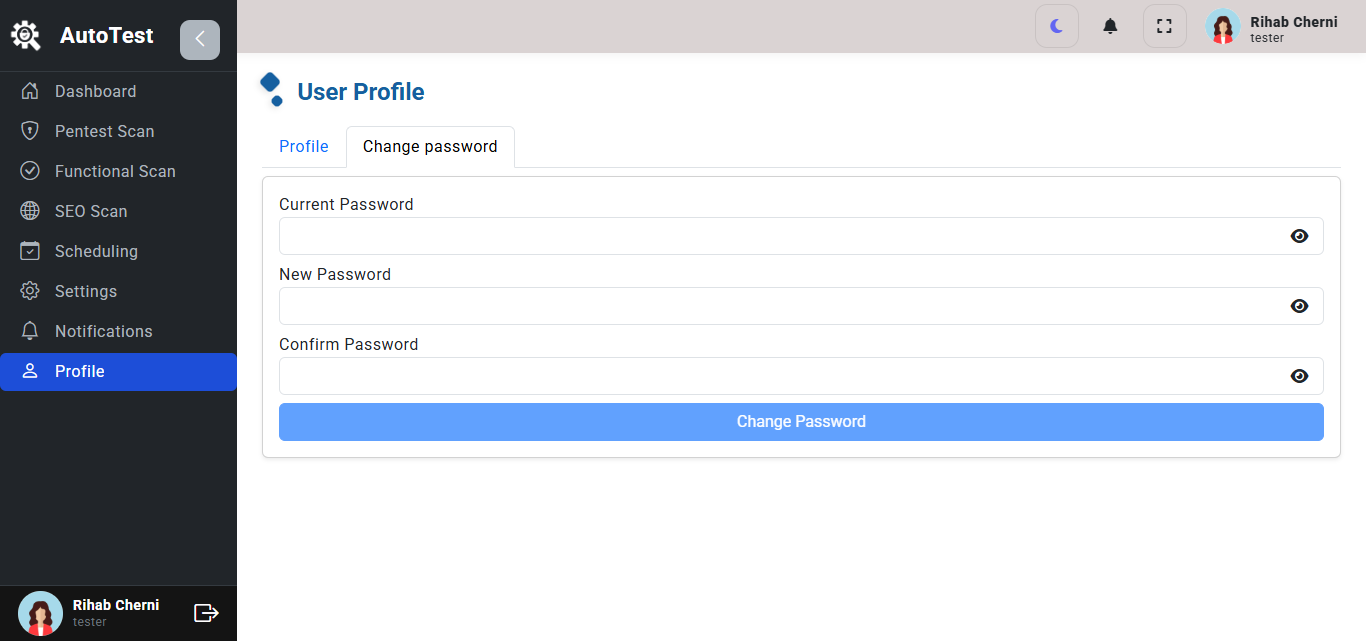
\includegraphics[width=0.9\linewidth]{chapitres/ch3Sp1/section/sprint1/img/interface/change-profile.png}
                    \caption{\centering Interface de modification du mot de passe}
                    \label{fig:password-update}
                \end{figure}
                 \vspace{-0.6cm}
                \begin{figure}[H]
                    \centering
                    \begin{subfigure}[b]{0.32\linewidth}
                        \centering
                        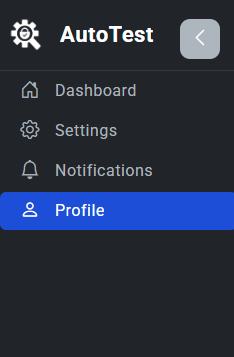
\includegraphics[width=0.9\linewidth]{chapitres/ch3Sp1/section/sprint1/img/interface/0-permission-sidebar.PNG}
                        \caption{Sans droits d'accès}
                    \end{subfigure}
                    \hfill
                    \begin{subfigure}[b]{0.32\linewidth}
                        \centering
                        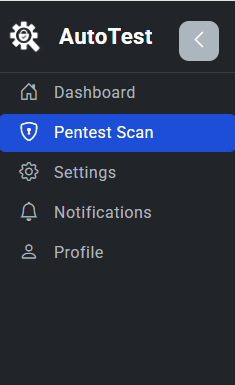
\includegraphics[width=0.9\linewidth]{chapitres/ch3Sp1/section/sprint1/img/interface/1-permssion.PNG}
                        \caption{Avec permissions de sécurité}
                    \end{subfigure}
                    \hfill
                    \begin{subfigure}[b]{0.32\linewidth}
                        \centering
                        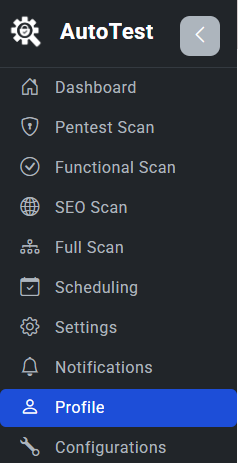
\includegraphics[width=0.9\linewidth]{chapitres/ch3Sp1/section/sprint1/img/interface/all-permssion-sidebar.PNG}
                        \caption{Avec toutes les permissions}
                    \end{subfigure}
                    \caption{Menu latéral de Testeur}
                    \label{fig:sidebar}
                \end{figure}
                \begin{figure}[H]
                    \centering
                    \begin{subfigure}[b]{0.48\linewidth}
                        \centering
                        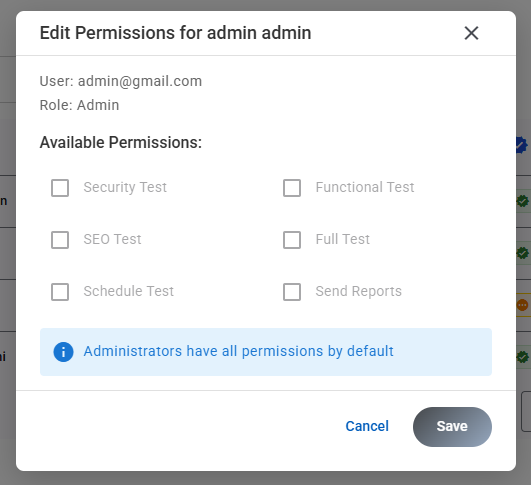
\includegraphics[width=\linewidth]{chapitres/ch3Sp1/section/sprint1/img/interface/edit-permission-admin.PNG}
                        \caption{\centering Interface d’édition des permissions pour l’administrateur}
                        \label{fig:subfig-admin}
                    \end{subfigure}
                    \hfill
                    \begin{subfigure}[b]{0.51\linewidth}
                        \centering
                        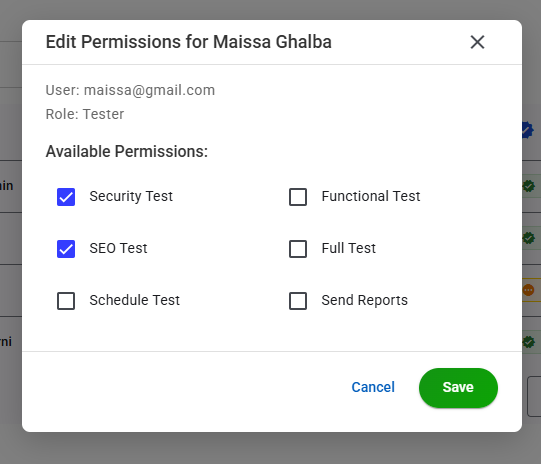
\includegraphics[width=\linewidth]{chapitres/ch3Sp1/section/sprint1/img/interface/edit-permission-users.PNG}
                        \caption{\centering Interface d’édition des permissions pour le testeur}
                        \label{fig:subfig-testeur}
                    \end{subfigure}
                    \hfill
                    \begin{subfigure}[b]{0.55\linewidth}
                        \centering
                        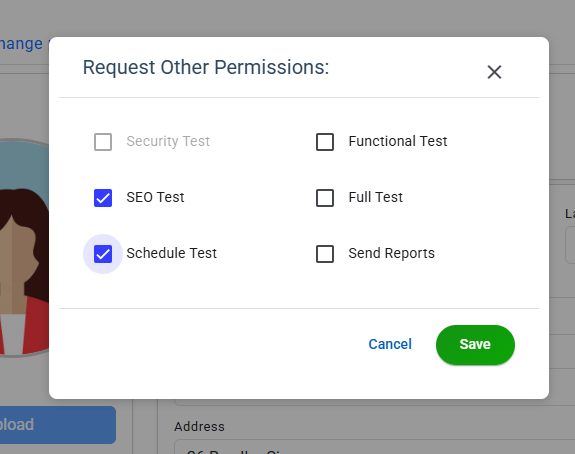
\includegraphics[width=\linewidth]{chapitres/ch3Sp1/section/sprint1/img/interface/demande-perm.PNG}
                        \caption{\centering Demande de permissions supplémentaires pour le testeur}
                        \label{fig:subfig-demande}
                    \end{subfigure}
                    \caption{\centering Interfaces liées à la gestion des permissions}
                    \label{fig:permission-interfaces}
                \end{figure}
                \vspace{-0.3cm}
                \begin{figure}[H]
                    \centering
                    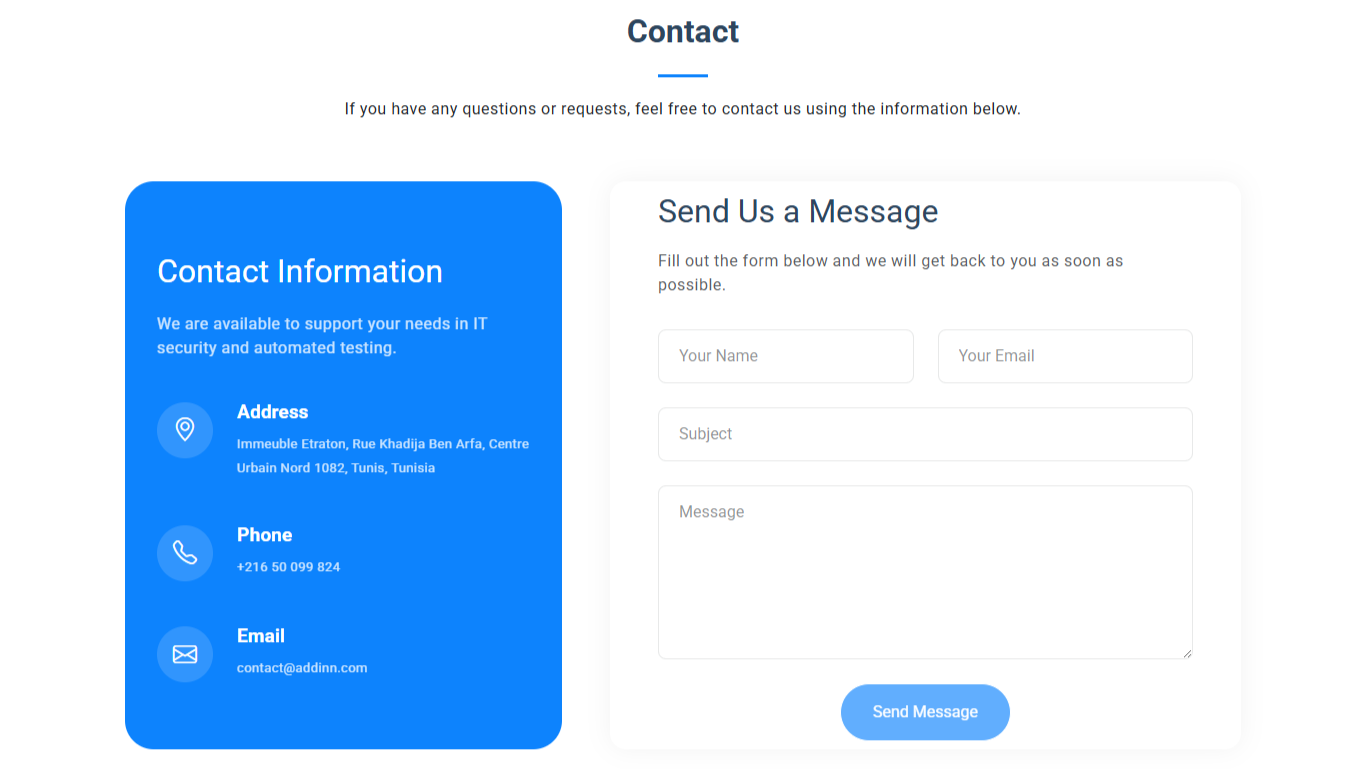
\includegraphics[width=\linewidth]{chapitres/ch3Sp1/section/sprint1/img/interface/contact.png}
                    \caption{\centering Interface de soumission de message de contact}
                    \label{fig:contact}
                \end{figure}
                \vspace{-0.6cm}
                \begin{figure}[H]
                    \centering
                    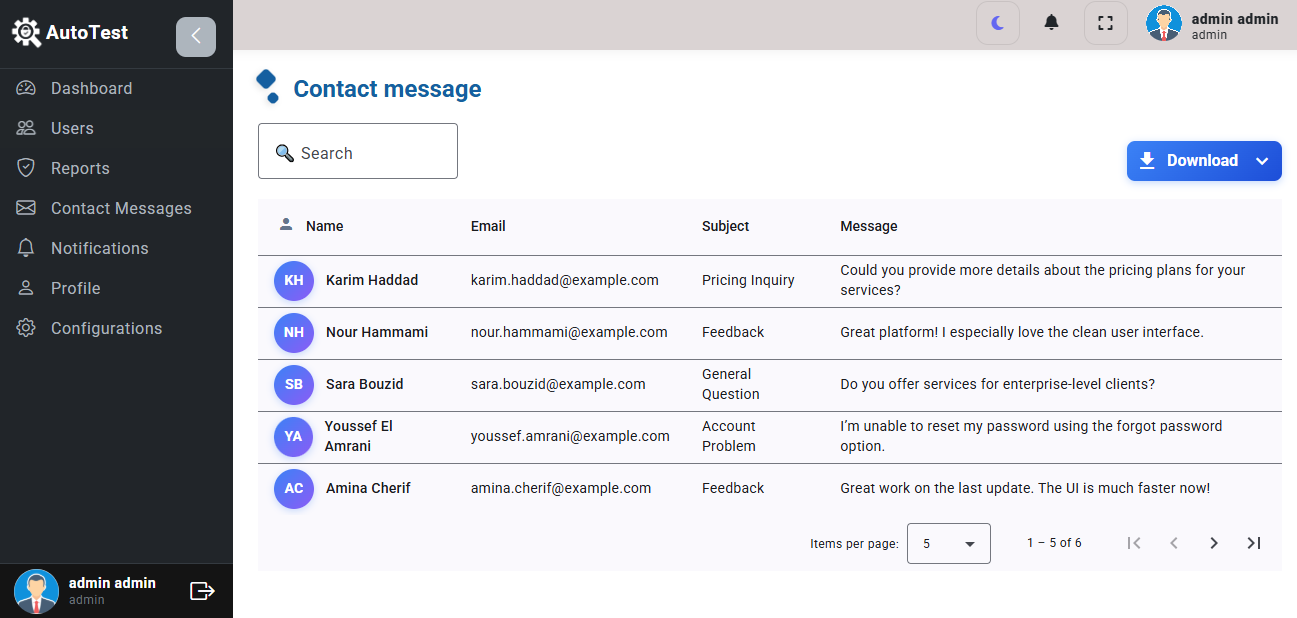
\includegraphics[width=0.9\linewidth]{chapitres/ch3Sp1/section/sprint1/img/interface/contact-liste.PNG}
                    \caption{\centering Interface d’administration: liste des messages reçus via le formulaire de contact} 
                    \label{fig:admin-contact-list}
                \end{figure}
                 \vspace{-0.2cm}
                
                \item \textbf{Sprint 1.2 : Tests de sécurité et notifications}
                
                Ce sprint a permis d’enrichir l’application en intégrant des fonctionnalités essentielles liées à la sécurité ainsi qu’à l’interaction avec les utilisateurs :
                    \begin{figure}[H]
                        \centering
                        \includegraphics[width=\textwidth]{}
                        \caption{Interface de configuration des paramètres de scan}
                        \label{fig:interface_parametres_scan}
                    \end{figure}
                
                        
                    \begin{figure}[H]
                        \centering
                        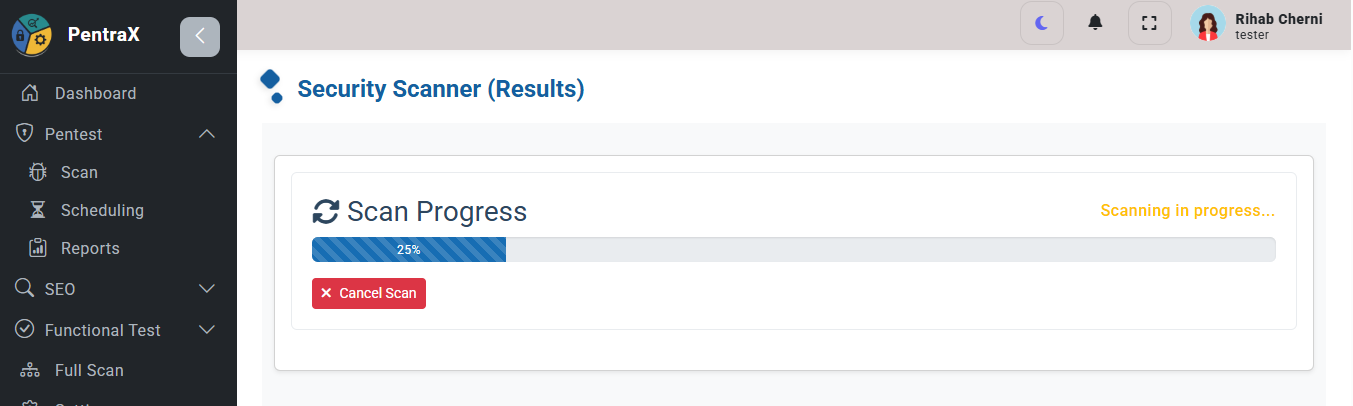
\includegraphics[width=\textwidth]{chapitres/ch3Sp1/section/sprint2/img/interface/prog.PNG}
                        \caption{Interface de suivi en temps réel des scans (WebSocket)}
                        \label{fig:interface_suivi_ws}
                    \end{figure}
    
                     \begin{figure}[H]
                        \centering
                        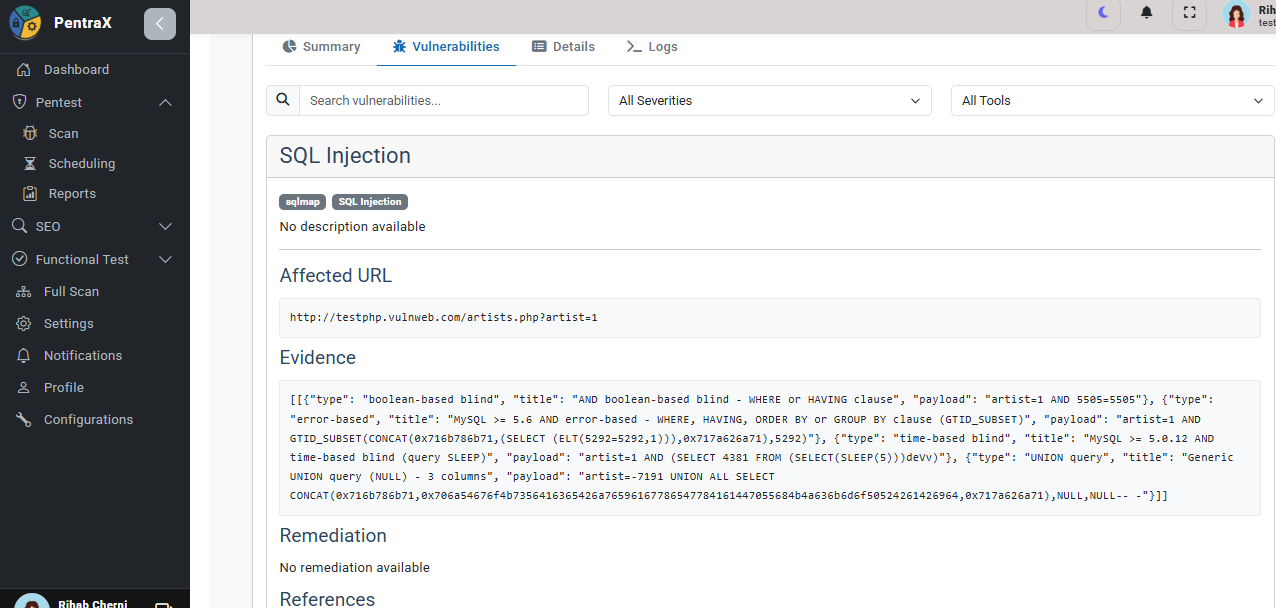
\includegraphics[width=\textwidth]{chapitres/ch3Sp1/section/sprint2/img/interface/vle.PNG}
                        \caption{Interface de visualisation des résultats de scan 2}
                        \label{fig:interface_resultats_scan2}
                    \end{figure} 
                    \begin{figure}[H]
                        \centering
                        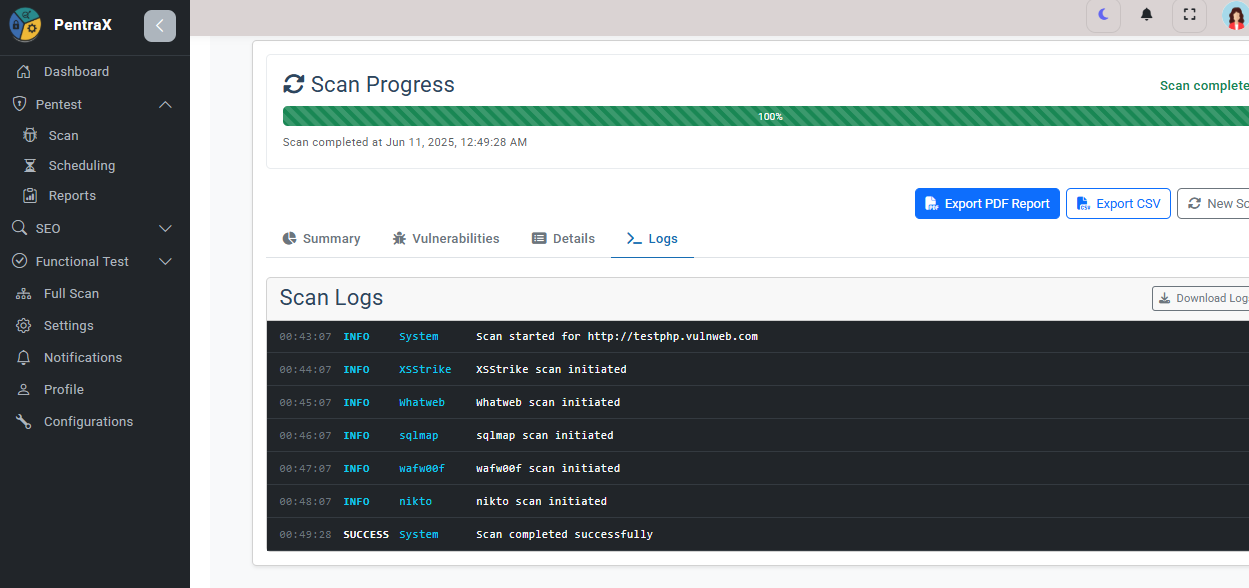
\includegraphics[width=\textwidth]{chapitres/ch3Sp1/section/sprint2/img/interface/logs.PNG}
                        \caption{Interface de visualisation des résultats de scan 3}
                        \label{fig:interface_resultats_scan2}
                    \end{figure} 
                    \begin{figure}[H]
                        \centering
                        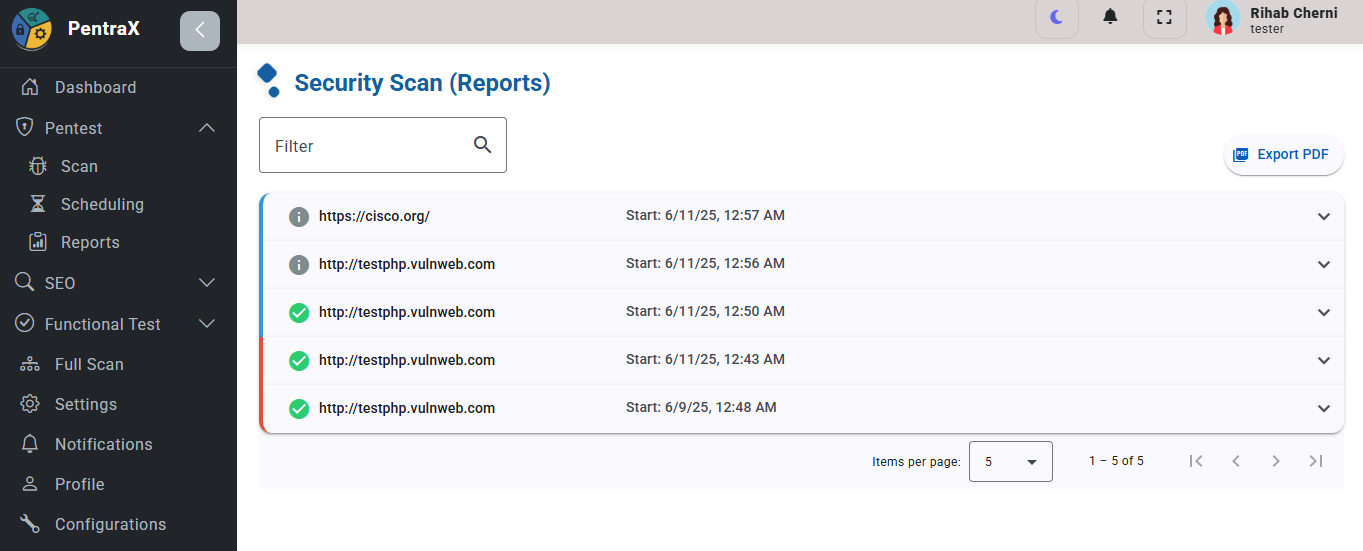
\includegraphics[width=\textwidth]{chapitres/ch3Sp1/section/sprint2/img/interface/table-sec.PNG}
                        \caption{Interface de l’historique des scans}
                        \label{fig:interface_historique_scans}
                    \end{figure}
    
                     \begin{figure}[H]
                        \centering
                        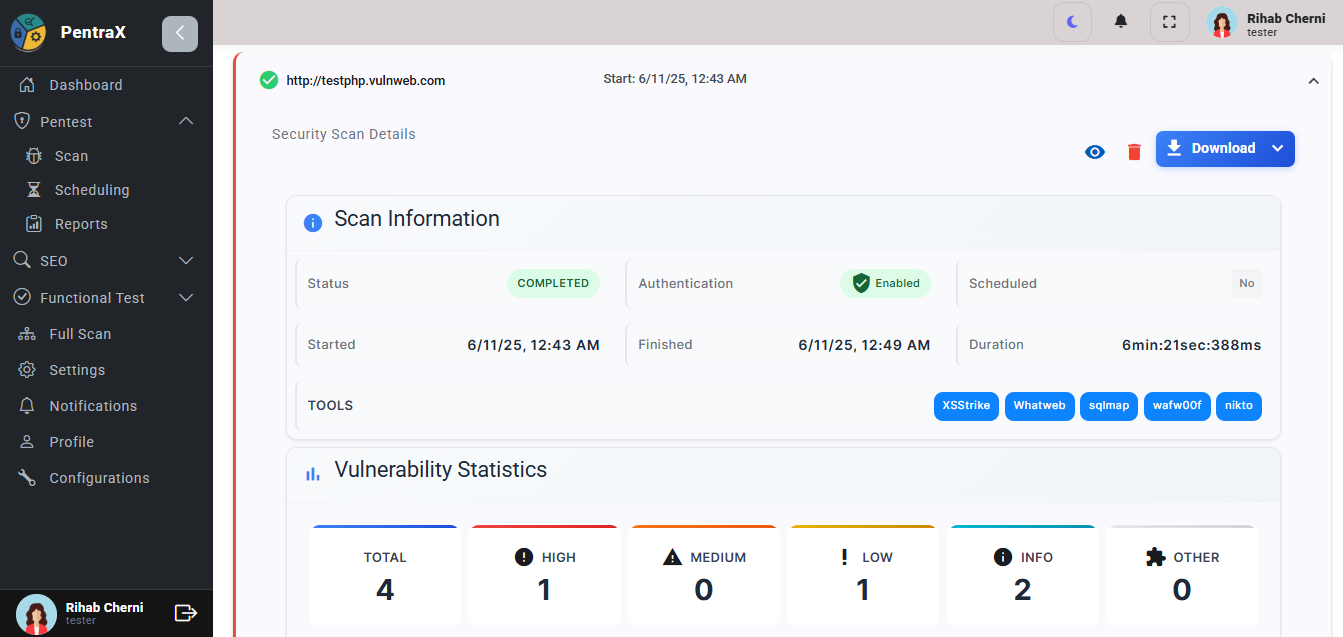
\includegraphics[width=\textwidth]{chapitres/ch3Sp1/section/sprint2/img/interface/details-sec1.PNG}
                        \caption{Interface de l’historique des scans (détails scan)}
                        \label{fig:interface_historique_details}
                    \end{figure}
                    \begin{figure}[H]
                        \centering
                        \includegraphics[width=0.4\textwidth]{}
                        \caption{Téléchargement des rapports}
                        \label{fig:interface_export_rapports}
                    \end{figure}
    
                \begin{figure}[H]
                    \centering
                    \begin{subfigure}[b]{\linewidth}
                        \centering
                        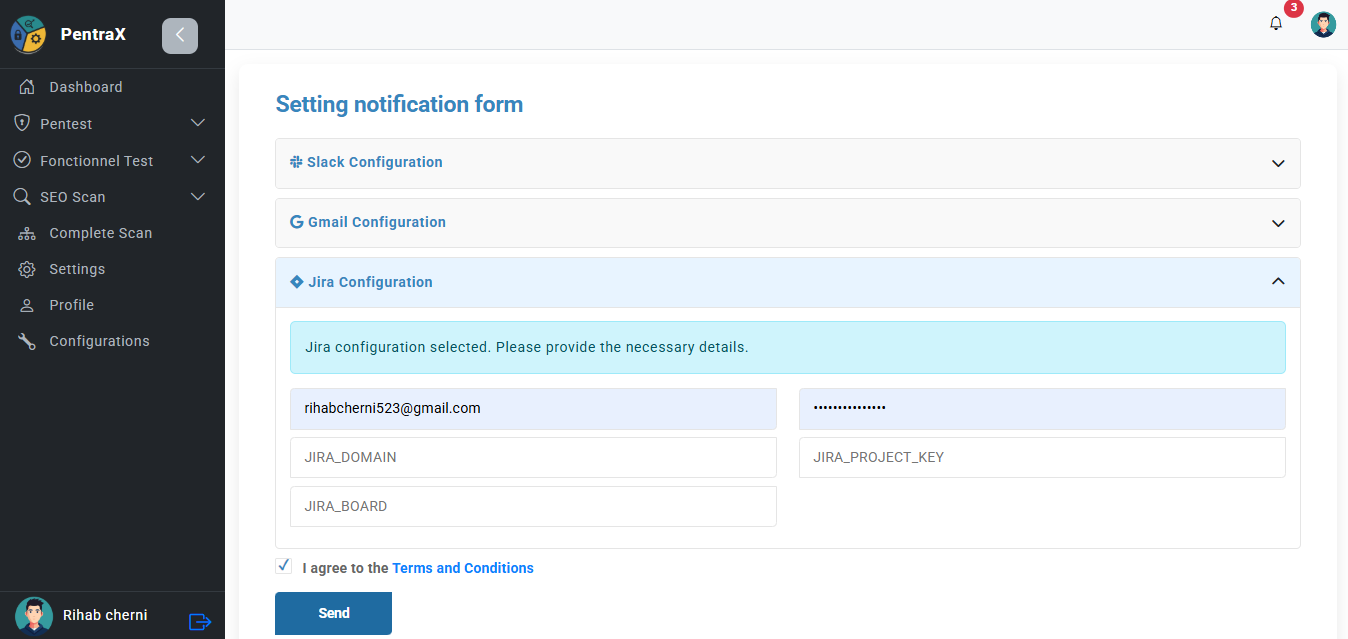
\includegraphics[width=\linewidth]{chapitres/ch3Sp1/section/sprint2/img/interface/configuration.PNG}
                        \caption{Interface de configuration}
                    \end{subfigure}
                    \hfill
                    \begin{subfigure}[b]{0.44\linewidth}
                        \centering
                        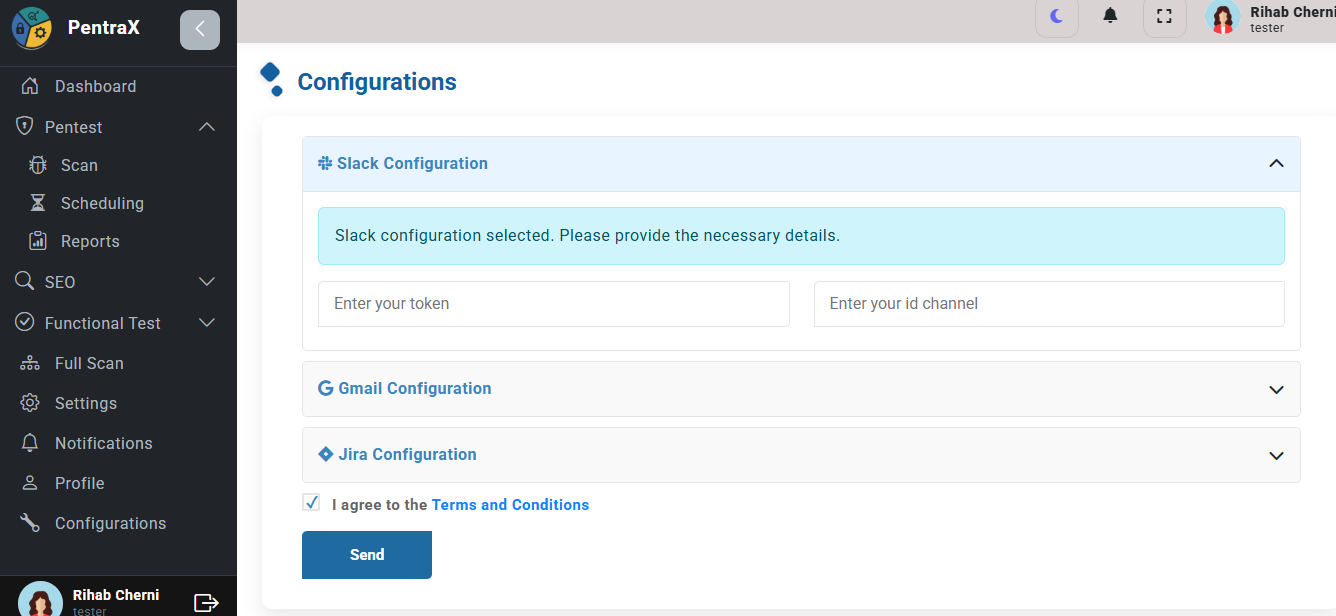
\includegraphics[width=\linewidth]{chapitres/ch3Sp1/section/sprint2/img/interface/cof-slack.PNG}
                        \caption{Configuration Slack}
                    \end{subfigure}
                    \hfill
                    \begin{subfigure}[b]{0.5\linewidth}
                        \centering
                        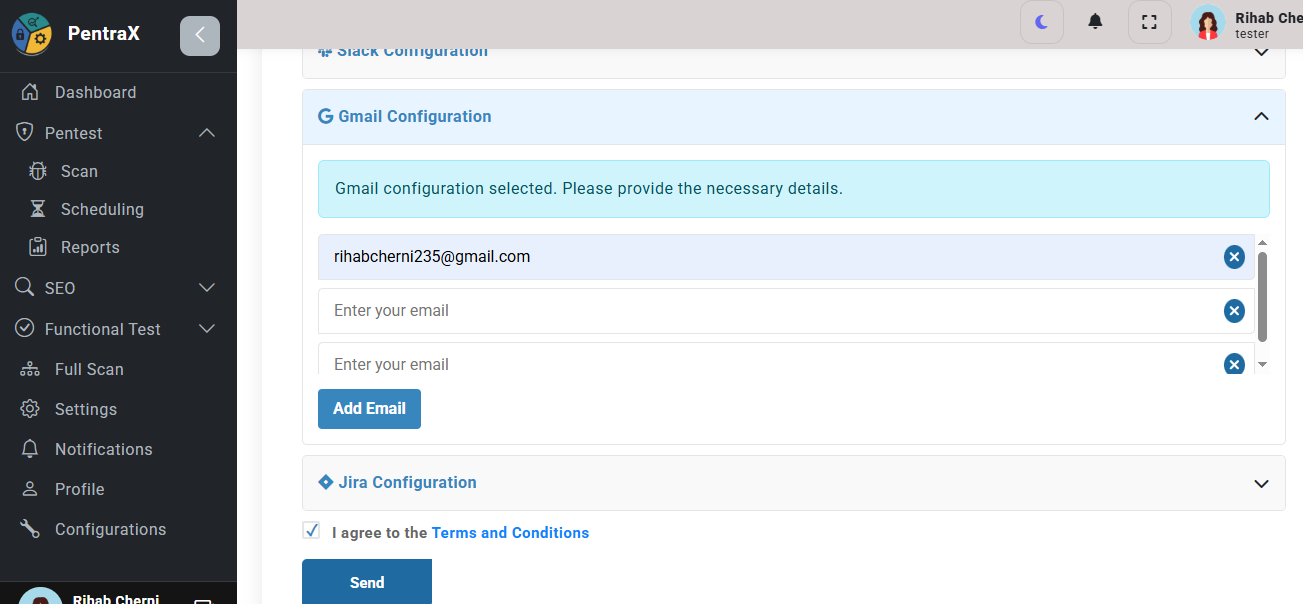
\includegraphics[width=\linewidth]{chapitres/ch3Sp1/section/sprint2/img/interface/cof-email.PNG}
                        \caption{Email}
                    \end{subfigure}
                    \hfill
                    \begin{subfigure}[b]{0.5\linewidth}
                        \centering
                        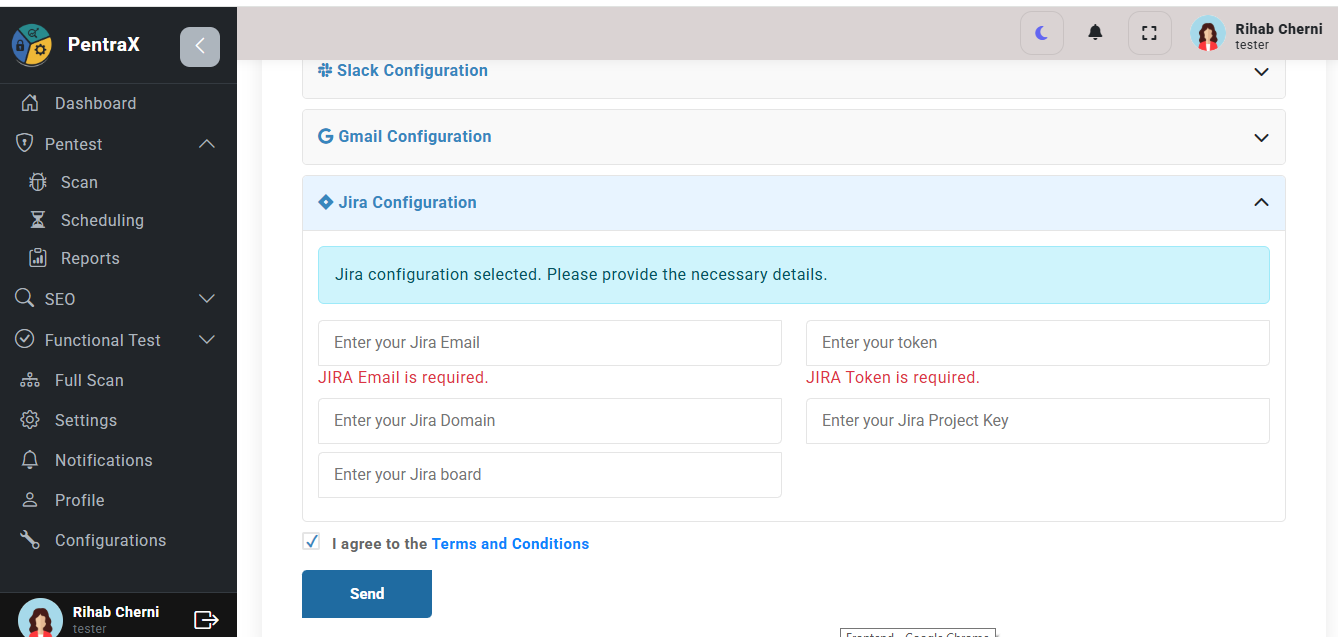
\includegraphics[width=\linewidth]{chapitres/ch3Sp1/section/sprint2/img/interface/cof-ira.PNG}
                        \caption{Configuration Jira}
                    \end{subfigure}
                    \hfill
                    \begin{subfigure}[b]{0.49\linewidth}
                        \centering
                        \includegraphics[width=0.42\linewidth]{}
                        \caption{Configuration formats et types d'envoi des rapports}
                    \end{subfigure}
                    \caption{Interface de paramétrage des canaux de diffusion}
                    \label{fig:fig:interface_parametrage_canaux}
                \end{figure}
                
                    \begin{figure}[H]
                        \centering
                        \includegraphics[width=\textwidth]{}
                        \caption{Interface d’intégration Jira}
                        \label{fig:interface_jira_integration}
                    \end{figure}
                        
                    \begin{figure}[H]
                        \centering
                        \includegraphics[width=\textwidth]{}
                        \caption{Interface de notification via Slack}
                        \label{fig:interface_slack_notification}
                    \end{figure}
                        
                    \begin{figure}[H]
                        \centering
                        \includegraphics[width=\textwidth]{}
                        \caption{Interface de notification par e-mail}
                        \label{fig:interface_email_notification}
                    \end{figure}
                        
                    \begin{figure}[H]
                        \centering
                        \includegraphics[width=\textwidth]{}
                        \caption{Interface de planification automatique des scans}
                        \label{fig:interface_planification_scan}
                    \end{figure}
                        
                    \begin{figure}[H]
                        \centering
                        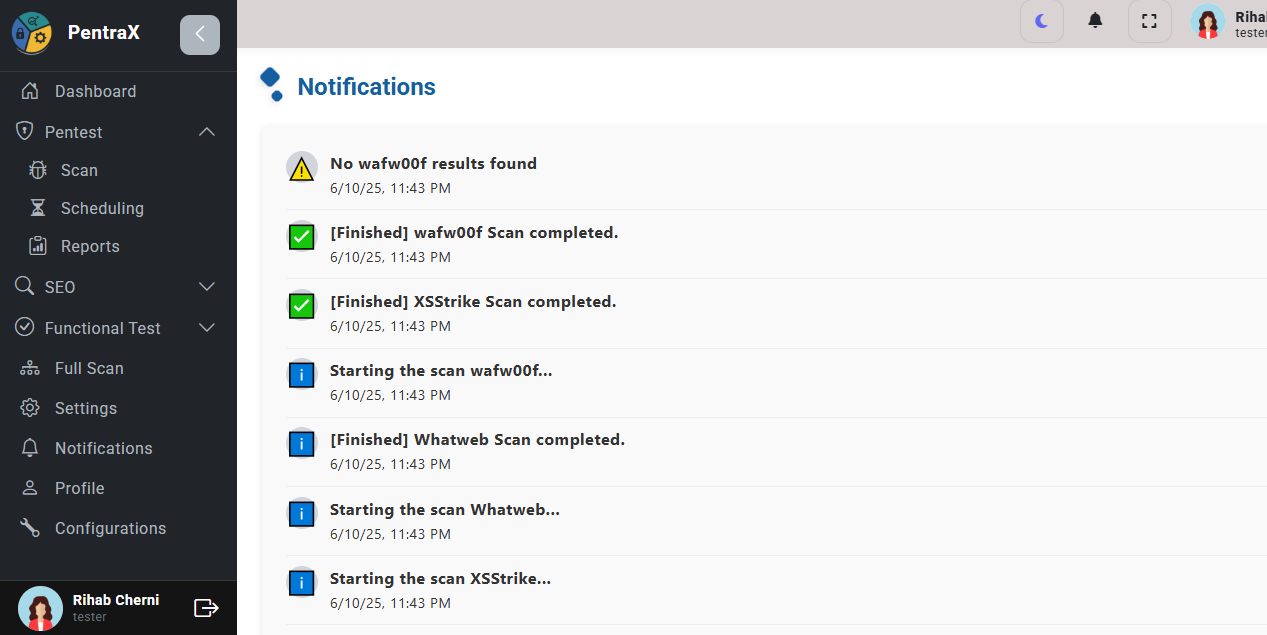
\includegraphics[width=\textwidth]{chapitres/ch3Sp1/section/sprint2/img/interface/Notifications.PNG}
                        \caption{Interface de gestion centralisée des notifications}
                        \label{fig:interface_notifications_config}
                    \end{figure}
    
    
    
    
                
            \end{enumerate}

    \textbf{\fontsize{16}{19}\selectfont  Release 2} :\\
            \begin{enumerate}[label=\Alph*]
                \item \textbf{Sprint 2.1} :
                \item \textbf{Sprint 2.2} :
            \end{enumerate}
    \end{justify}


% % \begin{figure}[H]
% %     \centering
% %     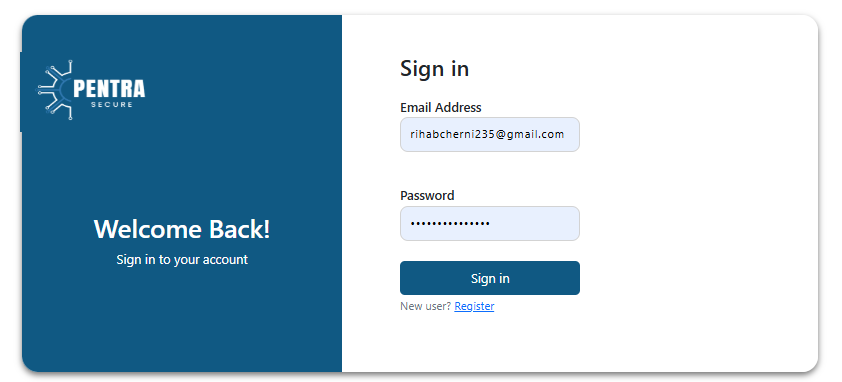
\includegraphics[width=\linewidth]{Annexe/PENTRA-V2/3.png}
% %     \caption{\centering Interface de lancement du scan repensée pour une meilleure compréhension des options}
% %     \label{fig:3}
% % \end{figure}
% % \vspace{-0.3cm}

% % \begin{figure}[H]
% %     \centering
% %     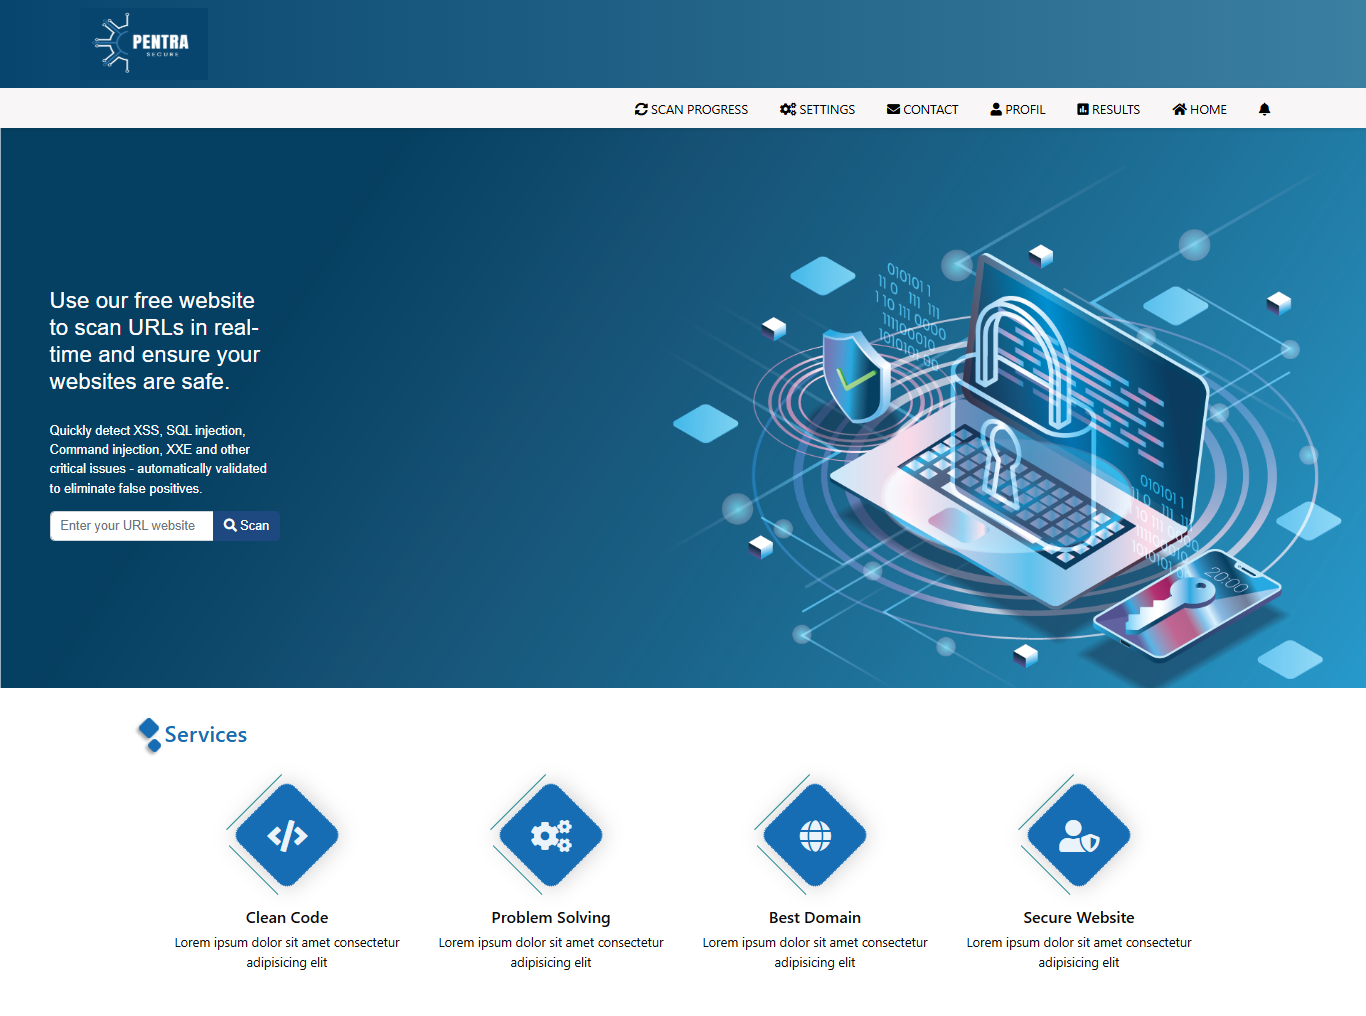
\includegraphics[width=\linewidth]{Annexe/PENTRA-V2/4.png}
% %     \caption{\centering Affichage unifié et clair de la progression des différents outils de scan}
% %     \label{fig:4}
% % \end{figure}
% % \vspace{-0.3cm}

% % \begin{figure}[H]
% %     \centering
% %     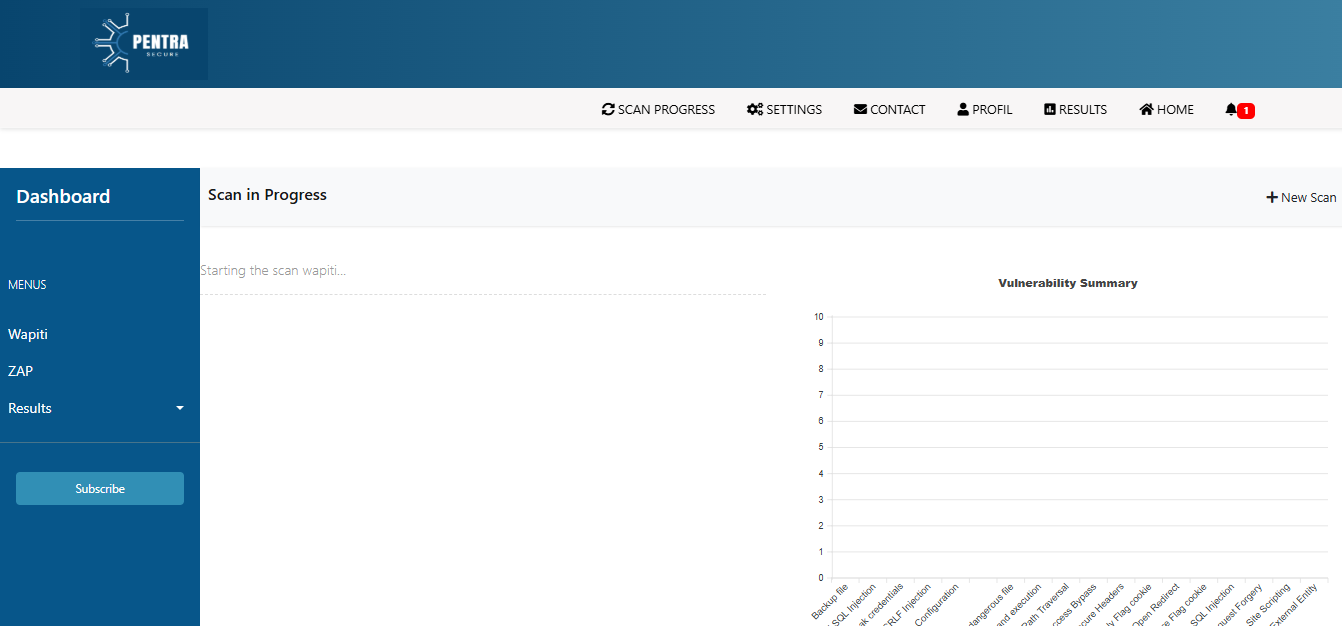
\includegraphics[width=\linewidth]{Annexe/PENTRA-V2/5.png}
% %     \caption{\centering Tableau de résultats amélioré avec filtres et tri dynamique}
% %     \label{fig:5}
% % \end{figure}
% % \vspace{-0.3cm}

% \begin{figure}[H]
%     \centering
%     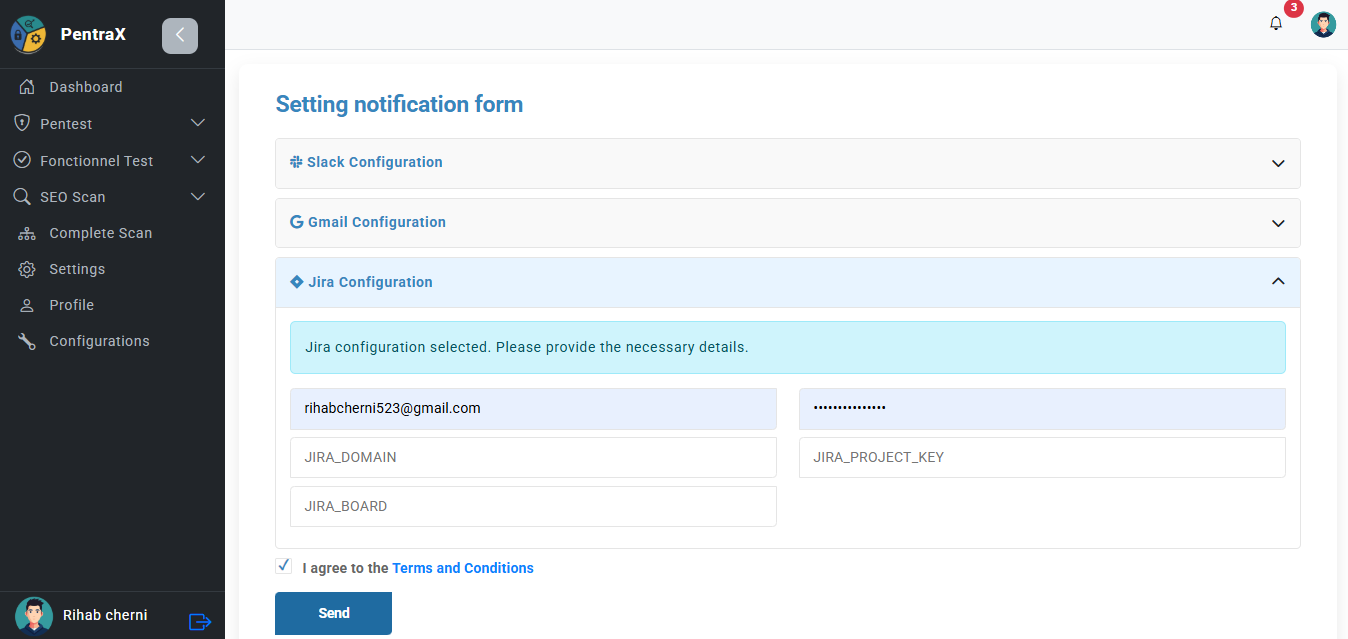
\includegraphics[width=\linewidth]{chapitres/ch3Sp1/section/sprint2/img/interface/configuration.PNG}
%     \caption{\centering Interface de configuration des notifications (Slack, Email, Jira)}
%     \label{fig:6}
% \end{figure}

% % \begin{figure}[H]
% %     \centering
% %     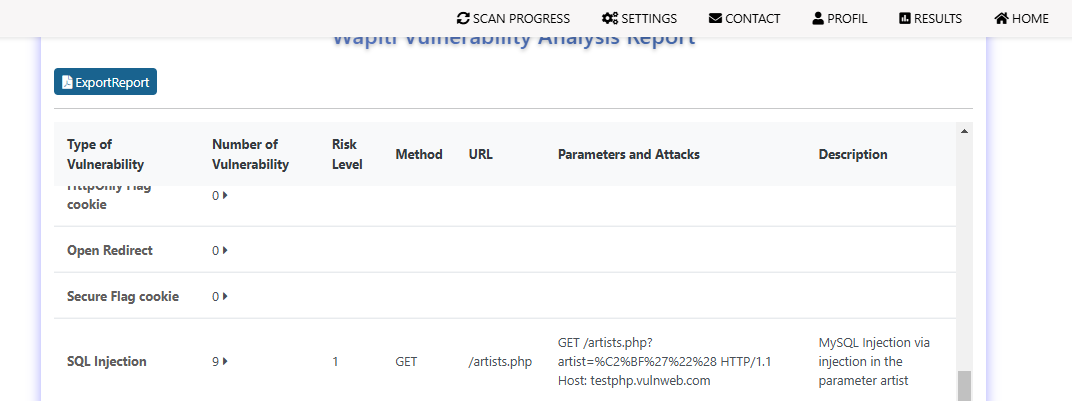
\includegraphics[width=\linewidth]{Annexe/PENTRA-V2/8.png}
% %     \caption{\centering Interface d'historique des rapports avec options de visualisation et téléchargement}
% %     \label{fig:8}
% % \end{figure}
% % \vspace{-0.8cm}

% % \begin{figure}[H]
% %     \centering
% %     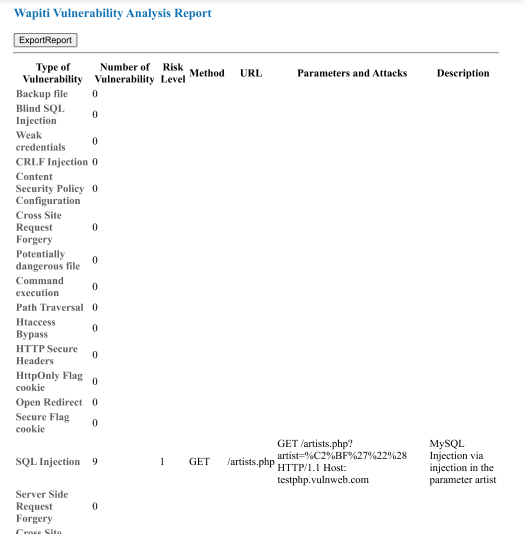
\includegraphics[width=\linewidth]{Annexe/PENTRA-V2/9.png}
% %     \caption{\centering Rapport PDF repensé avec une structure claire et un sommaire automatisé}
% %     \label{fig:9}
% % \end{figure}
% % \vspace{-0.8cm}

% % \begin{figure}[H]
% %     \centering
% %     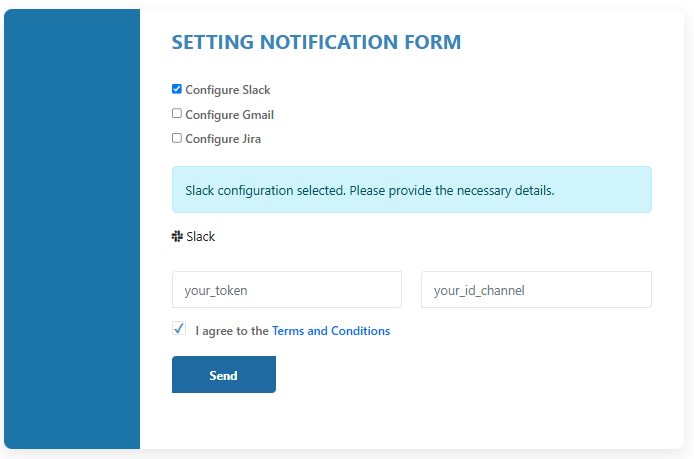
\includegraphics[width=\linewidth]{Annexe/PENTRA-V2/10.png}
% %     \caption{\centering Nouveau tableau de bord}
% %     \label{fig:10}
% % \end{figure}
% % \vspace{-0.8cm}